\chapter{Background \& Objectives}

In this chapter, the project itself will be discussed. There will be an emphasis on the preparation, analysis, and the processes that will be undertaken to complete the project.

\section{Background}

This section will discuss the preparation and background that has been completed for this project; it's split between 3 subsections for more straightforward navigation.

\subsection{Background Preparation} \label{BACKPREP}
Before the project started, there was some brief research into where and how someone would adopt cats. Most places offer an internet portal or web application that allows a user to find a cat they would like to adopt. With a background in Version Control, there was a git repository setup on GitHub. As I already had a project on Android with Instrumentation and Unit testing involved, I went and started researching the various Continuous Integration platforms that are available, after looking into Jenkins \cite{JENKINS} and Travis \cite{TRAVIS}, and Bitrise \cite{BITRISE}.

\subsection{Similar Systems}
I investigated multiple Android applications that were aimed at providing a platform for adoption agencies and centres to adopt out not only cats but all kinds of pets. I investigated the following Android based applications:

\begin{itemize}
    \item Pets Adoption: Adopt Dog, Cat or Post for Adoption \cite{PETSADOPTION}
    \item Pets Adoption: Adopt Dog, Cat and Other Pets \cite{PETSADOPTION1}
    \item Appets - Adopt a pet \cite{APPETS}
    \item Pet Adoption UK \cite{PETADOPTIONUK}
\end{itemize}

There was a distinct lack of single agency native Android applications,  where only one adoption charity operates, for example, the RSPCA \cite{RSPCA} and Cats Protection \cite{CATSPROTECTION} do not provide native Android applications. However, they do have well-structured websites. I took an in-depth look into their designs for their cat finding tools and used their websites as inspiration for what data to track for the individual cats that are up for adoption on my application. 

\subsection{Motivation and Interest}
I have a great interest in Android design due to studying it in my first semester of 3rd year, coupled with my desire to go and do something different to my year in industry and my future employment with the same employer, and Android-based project seemed ideal. I have a keen interest in general Software Engineering, and I decided that this project would allow me to apply all of the skills and techniques I have learnt at university and in my industrial year. The project provided significant challenges when it came to Continuous Integration and general development cycle elements, such as Android is a hard system to emulate unless using specific hardware, which I was not initially using.

\section{Analysis}
This section analyses the key problems, for the application as a problem that needs to be solved and the key objectives or stories that need to be completed to make this application feature complete.

\subsection{Key Problems}
The problem boils down into a few key ideas:
\begin{itemize}
    \item Prototype Design
    \item Data, and its protection (Section \ref{DATAPROTECTION} for protection, Section \ref{DATAIMPLEMENTATION} for the data part)
    \item Implementation of the application (Appendix Chapter \ref{IMPLEMENTATION})
    \item Version Control choice 
    \item Continuous Integration implementation
    \item Acquiring cat data
\end{itemize}

\subsubsection{Prototype Design}

There are numerous prototyping software choices, Adobe XD \cite{ADOBEXD} and FluidUI \cite{FLUIDUI} I have used previously but they both left something to be desired, with parts being either hard to use or locked behind a paywall. I found a web app called Figma \cite{FIGMA} that allows a student or person with an academic email that allows detailed prototyping and functional implementation for a prototype for free. Figma has detailed Material functions and makes life very easy when designing things for a UX environment, by allowing copies of a master object that changes all of its children objects.

\subsubsection{Version Control}
The need for version control boils down not to the fact that there is more than one contributor, but smooth interaction with the continuous integration,  the ability to revert broken changes, and quickly backup the application to a 3rd party source. The chosen 3rd party is GitHub \cite{GITHUB}, and it's an easy to use platform for project and repository development across multiple devices. I find it to be invaluable for its project boards for Kanban and issue tracking, alongside easy webhook integration for my Continuous Integration.

\subsubsection{Continuous Integration} \label{CI}
Continuous integration's benefits and usefulness was already mostly discussed in Section \ref{BACKPREP}. The choice and why it was picked is discussed here as opposed to its alternatives. The system chosen was Bitrise \cite{BITRISE}, due to the nature of Android development and free integration for Android Instrumentation tests with little setup, easy workflow management, and free, open-source build time Bitrise was the best platform for this project. Travis \cite{TRAVIS} was unable to perform it's own Android Emulation for Instrumentation testing due to the nature of the cloud computing docker container the tests run in, and its integration with Firebase Instrumentation Testing is lacking in the front of ease of use, and would mostly require extensive Bash scripting to get it to work correctly. Jenkins \cite{JENKINS} is very customise-able and allows a user to run tests on their systems, the downside of this is running the tests on their systems requires that system to be set correctly and stay set only continuously. A container wouldn't be feasible for Jenkins, due to the nature of Android Emulation so a physical hardware machine must be dedicated, alongside Bash/Groovy scripting to implement the Android test implementation. Due to the nature of Jenkins and Travis not being built for Android testing, it is not surprising that Bitrise seems like the best option.

\subsubsection{Cat Data}
The easiest way to get data was to take it from somewhere else, I spoke to Cats Protection \cite{CATSPROTECTION}, and got to speak with the Manager of their database and web systems, who promptly refused me access and permissions for images. Not wanting to get rejected from other charities as, my supervisor and I believed that was likely, I resorted to generating the data, I created a set of scripts taking in a set of predefined made up of data and produced them in a format that would be useful for the data. All cat images were sourced under the Pexels License \cite{PEXELSLICENSE}.

\subsubsection{Open Source and the License}
The project is open source so any charity, company, institution that may make use of the project can. Apache 2.0 \cite{APACHE2LICENSE} was the license of choice for this project as it looks to be the least obstructive license while still maintaining appropriate copyright protection, without providing any warranty.

\subsection{Objectives}
My Supervisor and I discussed my list of technical requirements (Appendix \ref{TECHREQUIREMENTS}) and boiled them down to some key stories that need to be produced for this project to be successful. Agreed-upon objectives are described in section \ref{STORIES} as stories, due to the nature of the process discussion I have discussed them there instead.

\subsection{Security and Data Protection} \label{DATAPROTECTION}
Security and Data Protection is paramount for multiple reasons, not only including the fact it's mandated by law and legislation from both the United Kingdom and the European Union but because we as Software Engineers have an ethical responsibility to protect people's data and act responsibly with the data that is collected.

In an effort to protect data, there should be required authentication, before a user can access any user data, this seems simple but should be stated that this was enforced using Firebase Firestore security rules. All user data should be stored using a unique identifier gained from Authentication software, using someone else's secure platform reduces the likely-hood that this software may cause a security breach, should be more ethical, for example using OAuth2 \cite{OAUTH} or the Firebase Authentication implementation \cite{FIREBASEAUTHENTICATION}.

It is feasibly possible that a user's data can be traced to an email, so access to the database should be restricted entirely to minimal developer access and ensuring that a minimal number of trusted individual(s) have access to it. The idea of restricting access increases general security by reducing entry points for hostile actors for the database. The database should be only accessed by a randomly generated string of characters as long as possible to remove the chance of someone guessing or cracking the password. All authentication should be handled by HTTPS encryption; if Firebase Authentication is used it correctly handles the encryption via HTTPS communication for authentication.

\subsection{User Identification}
The user can be anyone, as anyone can adopt a cat, with this in mind, it is clear that the application needs to have an emphasis on accessibility. With accessibility in mind, its discussed directly in my design as it's own Section (Section \ref{ACCESSIBILITYDESIGN}). 

Every user will need to be talked to over the phone to organise an appointment time and have their house checked for any obvious issues with a Cat living there, and these appointments would be conducted by an administrator; This reduces the likely hood of a Child or someone not able to care for a Cat finishing the adoption process.

\section{Process}

The process for application development that was implemented for this project was an agile approach in the form of a lighter version of Scrumban, which itself is an implementation of parts of both Scrum and Kanban. The project consists of multiple features or stories that are required to be implemented in the application. These stories represent a set part of work that must be completed for the application to be feature complete, each sprint may contain multiple stories, and a story may take multiple sprints based on its size discussed in Section \ref{STORIES}.

The aspects of Scrum that would be useful in an individual process is the sprints and planning when necessary approach, it allows me to focus on producing and delivering items of value regularly. A sprint consist of a 2-week block of time, where the next sprint is planned at the end of the last sprint and processes are improved as time continues. As part of the sprint process, I am performing a sprint retrospective after each sprint in an attempt to improve on estimates of work that can be completed, and improve on my general process of working. I believe that these retrospectives lead to a definite increase in productivity; sprint retrospectives are attached in the appendix \ref{SRINTRETROSPECTIVES}.

The aspects of Kanban that are employed are the Kanban board and the regular review process. The Kanban board allows me to produce a list of tasks and ensure that I do not get overwhelmed by sticking to a Work in Progress (WIP) point limit for tasks, of 1 in progress, so only 1 task may be worked on at a time. Kanban also lends itself to a regular review process that allows for continuous process improvement. GitHub has a feature called projects on a repository, which allows you to implement a Kanban board based on GitHub issues, I am using this for a public Kanban board per sprint, it is accessible here: \url{https://github.com/Pasarus/FelineAdoptionAgencyMajorProject/projects}.

\subsection{Stories}\label{STORIES}
    \begin{itemize}
        \item Design a working prototype of the application
        \item Refine the design of the prototype to ensure compliance with Material Design guidelines \cite{MATERIALDESIGNGUIDELINES}
        \item Utilise a functional Continuous Integration software (Bitrise \cite{BITRISE}) to perform routine tests and ensure the application works across multiple devices, resolutions, and API versions.
        \item Stick to the multiple coding standards for Python (Pep8), Kotlin (Coding Style Guidelines) and any other languages that have been chosen on the GitHub Wiki \url{https://github.com/Pasarus/FelineAdoptionAgencyMajorProject/wiki}
        \item Create a Cat Finder tool in the application that allows a person to find a cat to adopt similar to Cats Protection's find-a-cat \cite{CATSPROTECTION}. The tool should be a list, probably a RecyclerView that has a Material\gls{Card} that allows us to view some basic details and save the cat. The Card should include Image, Name, Age, and Location with more details available on tap, opening a more information screen, this should be done in line with the Material Guidelines \cite{MATERIALDESIGNGUIDELINES}
        \item A tool that displays detailed \gls{Card}s that represent the data of any Cat that has been saved by a user. These \gls{Card}s should be more detailed than those created in the Cat Finder tool, as these Cats are ones of keen interest to potential Adopters and should be featured as such.
        \item Login functionality that allows a user to sync data across devices (their saved cats and user data), allow a user to adopt a cat only when logged in and view their status for approval of the adoption of a cat.
        \item Utilise Google Firebase as storage for all data required by the application, with appropriate security enforced to ensure that user data is protected in line with current EU and UK data protection legislation including GDPR \cite{GDPRARTICLE1}
        \item Create adequate secondary screens to support the functionality of the application, including Settings, Help, Feedback, About, and My Account screens. When a user has logged in allow access to My Account otherwise request login before access is given because then data retrieval is possible.
        \item Create a sufficiently well-presented Landing/Home screen that allows a user to see their adoption statuses, and a featured cat so users can immediately see a cat, and their adoption statuses as easily as possible. Keeping a user in the app if possible if they accidentally click on it, would potentially lead to more users adopting, the user is likely to be more distracted by the immediate availability of a cute featured cat.
        \item Support Android 21+ for development in an aim to make the application available to at minimum 85\% of all Android users.
        \item Provide a correctly signed and as functional as possible release version of the application as an APK for Android.
    \end{itemize}
    
\subsection{Process of Adoption}
The process of adoption in the application should be relatively straightforward. A user should be logged in, and fill in their details before an adoption is added to the system, the necessary process is detailed in the Figure \ref{fig:adoptionProcess} which shows the decisions taken to get to an adoption appointment.

\begin{figure} [htbp!]
    \centering
    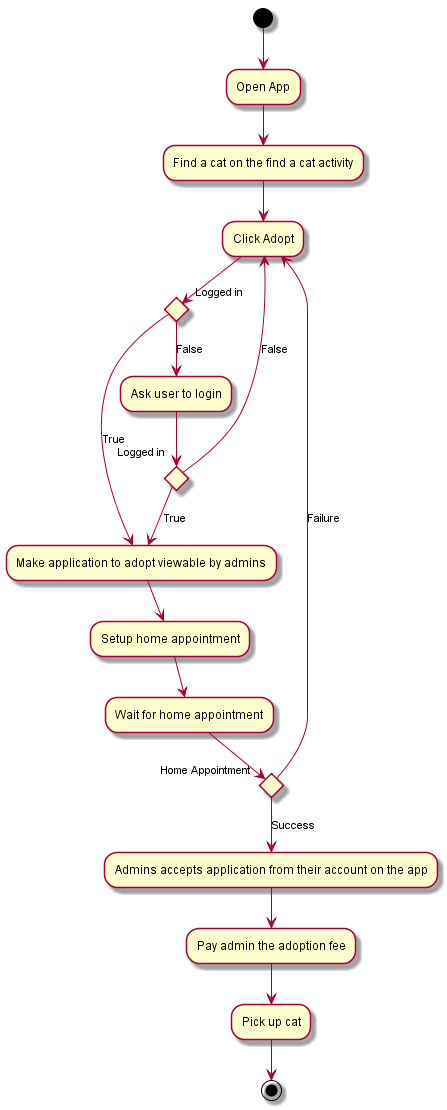
\includegraphics[scale=0.55]{Images/AdoptACat.png}
    \caption{The adoption UML activity diagram, for adopting a cat through the application}
    \label{fig:adoptionProcess}
\end{figure}